\documentclass[SingleSpace,12pt,Journal]{Serre_ASCE}
\usepackage[dvips]{graphicx}
\usepackage[dvipsnames]{xcolor}
\usepackage{amsmath}
\usepackage{amsfonts}
\usepackage{amssymb}
\usepackage[pdf]{pstricks}
\usepackage{psfrag}
\usepackage{pifont}
\usepackage{epstopdf}
%\usepackage{topcapt}
\usepackage{lscape}
\usepackage{amsthm}
\usepackage{pifont}
\usepackage{geometry}
\usepackage{fleqn}
\usepackage{txfonts}
\usepackage{wasysym}
\usepackage{lineno}
\usepackage{enumerate}
\usepackage{url}
\usepackage{times}
\usepackage{subfigure}
\usepackage{graphicx}
\usepackage{longtable}
%\usepackage{citeref}
\usepackage[skip=0pt]{caption}

% TIME ON EVERY PAGE AS WELL AS THE FILE NAME
\usepackage{fancyhdr}
\usepackage{currfile}
\usepackage[us,12hr]{datetime} % `us' makes \today behave as usual in TeX/LaTeX
\fancypagestyle{plain}{
\fancyhf{}
\rfoot{\small Draft Paper \\ File Name: {\currfilename} \\ Date: {\ddmmyyyydate\today} at \currenttime}
\lfoot{Page \thepage}
\renewcommand{\headrulewidth}{0pt}}
\pagestyle{plain}

\newcommand\solidrule[1][0.25cm]{\rule[0.5ex]{#1}{1pt}}
\newcommand\dashedrule{\mbox{%
  \solidrule[2mm]\hspace{2mm}\solidrule[2mm]}}

\begin{document}

\title{Behaviour of the Dam-Break Problem for the Serre Equations}

\author{
Jordan~Pitt,%
\thanks{Mathematical Sciences Institute, Australian National University, Canberra, ACT 0200, Australia, E-mail: Jordan.Pitt@anu.edu.au. The work undertaken by the first author was supported financially by an Australian National University Scholarship.}
\\
Christopher~Zoppou,\footnotemark[1]%
%
% Adding a second author with the same affiliation (still using \thanks):
\\
Stephen~G.~Roberts,\footnotemark[1]
}

\maketitle

\begin{abstract}

\end{abstract}

\KeyWords{dispersive waves, conservation laws, Serre equation, finite volume method, finite difference method}

\linenumbers

%--------------------------------------------------------------------------------
\section{Introduction} \label{intro} 

%--------------------------------------------------------------------------------
\section{Serre Equations}
\label{section:Serre Equations}
The Serre equations can derived as an approximation to the full Euler equations by depth integration similar to \cite{Su-Gardener-1969-536}. They can also be seen as an asymptotic expansion of the Euler equations \cite{Bonneton-Lannes-2009-16601}. The former is more consistent with the perspective from which numerical methods will be developed while the latter indicates the appropriate regions in which to use these equations as a model for fluid flow.
\begin{figure}[htb]
\begin{center}
\includegraphics[width=7.0cm]{pics/explainers/one-dimensional-axis_Serre.eps}
\end{center}
\caption{The notation used for one-dimensional flow governed by the Serre equation.}
\label{fig:Notation}
\end{figure}
The scenario under which the Serre approximation is made consists of a two dimensional $\textbf{x} = (x,z)$ fluid over a bottom topography as in Figure \ref{fig:Notation} acting under gravity. Consider a fluid particle at depth  $\xi(\textbf{x},t) = h(x,t) + z_b(x) - z$ below the water surface, see Figure \ref{fig:Notation}. Where the water depth is $h(x,t)$ and $z_b(x)$ is the bed elevation. The fluid particle is subject to the pressure, $p(\textbf{x},t)$ and  gravitational acceleration, $\textbf{g} = (0,g)^T$ and has a velocity $\textbf{u} = (u(\textbf{x},t),w(\textbf{x},t))$,  where $u(\textbf{x},t)$ is the velocity in the $x$-coordinate and $w(\textbf{x},t)$ is the velocity in the $z$-coordinate and $t$ is time. Assuming that $z_b(x)$ is constant the Serre equations read \cite{Guyenne-etal-2014-169}
\begin{linenomath*}
\begin{subequations}\label{eq:Serre_nonconservative_form}
\begin{gather}
\dfrac{\partial h}{\partial t} + \dfrac{\partial (\bar{u}h)}{\partial x} = 0
\label{eq:Serre_continuity}
\end{gather}
\begin{gather}
\underbrace{\underbrace{\dfrac{\partial (\bar{u}h)}{\partial t} + \dfrac{\partial}{\partial x} \left ( \bar{u}^2h + \dfrac{gh^2}{2}\right )}_{\text{Shallow Water Wave Equations}} + \underbrace{\dfrac{\partial}{\partial x} \left (  \dfrac{h^3}{3} \left [ \dfrac{\partial \bar{u} }{\partial x} \dfrac{\partial \bar{u}}{\partial x} - \bar{u} \dfrac{\partial^2 \bar{u}}{\partial x^2}  - \dfrac{\partial^2 \bar{u}}{\partial x \partial t}\right ] \right )}_{\text{Dispersion Terms}} = 0.}_{\text{Serre Equations}}
\label{eq:Serre_momentum}
\end{gather}
\end{subequations}
\end{linenomath*}
Where $\bar{u}$ is the average of $u$ over the depth of water. 
\subsection{Conservation of mass and momentum}
The Serre equations are based on conservation of mass and momentum, thus our numerical methods should reflect this property. The total of a quantity $q$ in a system is measured by

\begin{gather}
\label{eqn:Condef}
\mathcal{C}_q(t) = \int_{-\infty}^{\infty} q\, dx
\end{gather}
so that we have for all $t$ both $\mathcal{C}_{h}(0) = \mathcal{C}_{h}(t)$ and $\mathcal{C}_{\bar{u}h}(0) = \mathcal{C}_{\bar{u}h}(t)$ representing conservation of mass and momentum respectively.

\subsection{Hamiltonian}

The Serre equations admit a Hamiltonian \cite{Li-Y-2002,Hank-etal-2010-2034,Green-Naghdi-1976-237}

\begin{gather}
\label{eqn:Hamildef}
\mathcal{H}(t) = \frac{1}{2}\int_{-\infty}^{\infty} hu^2 + gh^2 + \frac{h^3}{3} \left(\frac{\partial u}{\partial x}\right)^2\, dx
\end{gather}
where the bar over $u$ has been dropped to simplify notation. The Hamiltonian is such that $\mathcal{H}(t) = \mathcal{H}(0)$ for all times $t$.

We can calculate this numerically by partitioning the total integral into cell-wise integrals. The cell-wise integral can then be calculated by quartic interpolation utilising neighbouring cells and then applying Gaussian quadrature with $3$ points over the cell to get a sufficiently high order method to calculate the Hamiltonian, in particular this method is at least third order accurate for the $\partial u / \partial x$ term. 
%--------------------------------------------------------------------------------
\section{Direct Numerical Methods} 
\label{sec:DirNumMet}
%--------------------------------------------------------------------------------
The presence of the mixed spatial temporal derivatives in the momentum equation \eqref{eq:Serre_momentum} makes the Serre equations difficult to solve with standard numerical methods. A naive way to avoid this is to approximate \eqref{eq:Serre_momentum} by finite differences and the results of this are presented here. To facilitate this a uniform grid in space will be used with $\Delta x  = x_{i+1} - x_i$ for all $i$. Quantities evaluated at these grid points will be denoted by subscripts for example $h_i = h(x_i)$. The grid in time is also uniform and will be denoted by superscripts for example $h^n = h(t^n)$, note that $h^n$ is a function in space. 
\subsection{Finite Difference Appximation to Conservation of Momentum Equation} 
\label{subsec:FDA2conmom}
In [][Zoppou thesis/my work] it was demonstrated that an efficient numerical scheme for the Serre equations must be at least second-order accurate thus the derivatives in \eqref{eq:Serre_momentum} will be approximated by second-order finite differences. Firstly \eqref{eq:Serre_momentum} must be expanded, making use of \eqref{eq:Serre_continuity} one obtains
\begin{linenomath*}
\begin{subequations}
\begin{gather}
h\dfrac{\partial u}{\partial t} + X - h^2\frac{\partial^2 u}{\partial x \partial t} - \frac{h^3}{3}\frac{\partial^3 u}{\partial x^2 \partial t}  =0 
\label{eq:expandedu}
\end{gather}
where $X$ contains only spatial derivatives and is
\begin{gather}
X = uh\frac{\partial u}{\partial x} + gh\frac{\partial h}{\partial x} + h^2\frac{\partial u}{\partial x}\frac{\partial u}{\partial x} + \frac{h^3}{3}\frac{\partial u}{\partial x}\frac{\partial^2 u}{\partial x^2} - h^2u\frac{\partial^2 u}{\partial x^2}- \frac{h^3}{3}u\frac{\partial^3 u}{\partial x^3} .
\end{gather}
\end{subequations}
\end{linenomath*} Taking the second-order centred finite difference approximation to the spatial and temporal derivatives for \eqref{eq:expandedu} after some rearranging gives
\begin{linenomath*}
\begin{gather}
h^{n}_iu^{n+1}_i - \left(h^{n}_i\right)^2 \left(\frac{u^{n+1}_{i+1} -u^{n+1}_{i-1} }{2 \Delta x}\right) - \frac{\left(h^{n}_i\right)^3}{3}\left(\frac{u^{n+1}_{i+1} - 2u^{n+1}_{i} + u^{n+1}_{i-1} }{\Delta x^2}\right) = - Y^n_i 
\label{eq:expandedutdisc3}
\end{gather}
\end{linenomath*}
where
\begin{linenomath*}
\begin{gather*}
Y_i^n = 2\Delta tX_i^{n} - h_i^{n}u_i^{n-1} + \left(h_i^{n}\right)^2\left(\frac{u^{n-1}_{i+1} -u^{n-1}_{i-1} }{2 \Delta x}\right) + \frac{\left(h_i^{n}\right)^3}{3}\left(\frac{u^{n-1}_{i+1} - 2u^{n-1}_{i} + u^{n-1}_{i-1} }{\Delta x^2}\right) .
\label{eq:expandfactor Xp}
\end{gather*}
\end{linenomath*}
Equation \eqref{eq:expandedutdisc3} can be rearranged into a tri-diagonal matrix that updates $u$ given its current and previous values. So that
\begin{linenomath*}
\begin{gather}
\left[\begin{array}{c}
 u^{n+1}_0 \\
 \vdots \\
 u^{n+1}_m \end{array}\right]
 = A^{-1} \left[\begin{array}{c}
  -Y^n_0 \\
  \vdots \\
  -Y^n_m \end{array}\right] =: \mathcal{G}_u\left(\boldsymbol{u}^n,\boldsymbol{h}^n, \boldsymbol{u}^{n-1},\boldsymbol{h}^{n-1}, \Delta x, \Delta t \right).
\label{eq:FDcentforu}
\end{gather}
\end{linenomath*}
In particular this is an explicit [?] numerical method for \eqref{eq:Serre_momentum}, that requires the current and previous values of $h$ and $u$.


\subsection{The Lax Wendroff Method for Conservation of Mass Equation}
\label{section:}
Because the conservation of mass equation \eqref{eq:Serre_continuity} has no mixed derivative term standard numerical techniques for conservation laws can be used. In particular the Lax-Wendroff method can be used as done by \citeN{El-etal-2006}, here we present the method in replicable detail.

Note that \eqref{eq:Serre_continuity} is in conservative law form for $h$ where the flux is $uh$. Thus using the previously defined spatio-temporal discretisation the two step Lax-Wendroff update[] for $h$ is
\begin{linenomath*}
\begin{gather}
h^{n + 1/2}_{i+ 1/2} = \frac{1}{2}\left(h^{n}_{i+1} + h^{n}_i\right) - \frac{\Delta t}{2\Delta x}\left(u^n_{i+1}h^n_{i+1} - h^n_{i}u^n_{i}\right),
\end{gather}
\begin{gather}
h^{n + 1/2}_{i- 1/2} = \frac{1}{2}\left(h^{n}_{i} + h^{n}_{i-1}\right) - \frac{\Delta t}{2\Delta x}\left(u^n_{i}h^n_{i} - h^n_{i-1}u^n_{i-1}\right),
\end{gather}
\begin{gather}
h^{n+1}_i = h^{n}_i - \frac{\Delta t}{\Delta x}\left(u^{n + 1/2}_{i+ 1/2}h^{n + 1/2}_{i+ 1/2} - u^{n + 1/2}_{i- 1/2}h^{n + 1/2}_{i- 1/2}\right).
\label{eq:LW4h}
\end{gather}
\end{linenomath*}
To calculate $u^{n + 1/2}_{i \pm 1/2}$ first $u$ is advanced in time by $\mathcal{G}_u$ then using linear interpolation in both space and time gives
\begin{gather}
u^{n + 1/2}_{i+ 1/2} = \frac{u^{n+1}_{i+1} + u^{n}_{i+1} + u^{n+1}_{i} + u^{n}_{i} }{4},
\end{gather}
\begin{gather}
u^{n + 1/2}_{i- 1/2} = \frac{u^{n}_{i} + u^{n}_{i} + u^{n+1}_{i-1}+ u^{n}_{i-1} }{4}.
\end{gather}
Thus we have the following update scheme
\begin{linenomath*}
\begin{gather}
\left[ \begin{array}{l}
\boldsymbol{h}^{n+1} \\
\boldsymbol{u}^{n+1}
 \end{array}\right] = \mathcal{E}\left(\boldsymbol{u}^n,\boldsymbol{h}^n, \boldsymbol{u}^{n-1},\boldsymbol{h}^{n-1}, \Delta x, \Delta t \right). 
\end{gather}
\end{linenomath*}

%--------------------------------------------------------------------------------
\subsection{Second Order Naive Finite Difference Method}
%--------------------------------------------------------------------------------
Here we also present a completely naive method for comparative purposes, to do this we apply the procedure used above on \eqref{eq:Serre_momentum} to \eqref{eq:Serre_continuity}. Thus the derivatives were first expanded then approximated by second order centered finite differences after rearranging this to give an update formula we obtain
\begin{linenomath*}
\begin{gather}
h^{n+1}_i = h^{n-1}_i - \Delta t \left(u^{n}_{i}\frac{h^{n}_{i+1} - h^{n}_{i-1}}{\Delta x} + h^{n}_{i}\frac{u^{n}_{i+1} - u^{n}_{i-1}}{\Delta x}\right).
\end{gather}
\end{linenomath*}
Preforming this update for all $i$ will be denoted by $\mathcal{G}_h\left(\boldsymbol{u}^n,\boldsymbol{h}^n,\boldsymbol{h}^{n-1} ,\Delta x, \Delta t \right)$.
Thus we get the naive second-order centred finite difference method for the Serre equations
\begin{linenomath*}
\begin{gather}
\left.
\begin{array}{l l}
\boldsymbol{h}^{n+1}&=\mathcal{G}_h\left(\boldsymbol{u}^n,\boldsymbol{h}^n, \Delta x, \Delta t \right) \\
\boldsymbol{u}^{n+1}&=\mathcal{G}_u\left(\boldsymbol{u}^n,\boldsymbol{h}^n, \boldsymbol{u}^{n-1},\boldsymbol{h}^{n-1}, \Delta x, \Delta t \right)
\end{array} \right\rbrace \mathcal{G}\left(\boldsymbol{u}^n,\boldsymbol{h}^n, \boldsymbol{u}^{n-1},\boldsymbol{h}^{n-1}, \Delta x, \Delta t \right).
\end{gather}
\end{linenomath*}
%-------------------------------------------------------------------------------- 
\section{Conservative Form of The Serre Equations}
To overcome the aforementioned difficulty of mixed derivatives the Serre equations \eqref{eq:Serre_nonconservative_form} can be reformulated into conservative form. This is accomplished by the introduction of a new quantity \cite{Hank-etal-2010-2034,Zoppou-2014}
\begin{linenomath*}
\begin{gather}
\label{eq:Gdefinition}
G = uh - h^2 \dfrac{\partial h}{\partial x} \dfrac{\partial u}{\partial x} - \frac{h^3}{3} \dfrac{\partial^2 u}{\partial x^2}.
\end{gather}
\end{linenomath*}
Consequently, \eqref{eq:Serre_nonconservative_form} can be rewritten as
\begin{linenomath*}
\begin{subequations}
\begin{gather}
\dfrac{\partial h}{\partial t} + \dfrac{\partial (uh)}{\partial x} = 0
\label{eq:Serrecon_continuity}
\end{gather}
and
\begin{gather}
\dfrac{\partial G}{\partial t} + \dfrac{\partial}{\partial x}\left(Gu + \dfrac{gh^2}{2} - \dfrac{2h^3}{3}\dfrac{\partial u}{\partial x}\dfrac{\partial u}{\partial x}\right) = 0.
\label{eq:Serrecon_momentum}
\end{gather}
\label{eq:Serrecon}
\end{subequations}
\end{linenomath*}

\subsection{A Hybrid Finite Difference-Volume Method for Serre Equations in Conservative Form}
\label{section:hybridmethod}
%--------------------------------------------------------------------------------
The conservative form \eqref{eq:Serrecon} allows for a wider range of numerical techniques such as finite element methods \cite{Guyenne-etal-2014-169} and finite volume methods \cite{Hank-etal-2010-2034,Zoppou-2014}. In this paper the first ($\mathcal{V}_1$), second ($\mathcal{V}_2$) and third-order ($\mathcal{V}_3$) finite difference-volume methods (FDVM) of [] will be used. These have been validated and their order of accuracy confirmed.

\subsection{Stability Condition} 
To ensure stability of the FDVMs the time-step $\Delta t$ must satisfy the Courant-Friedrichs-Lewy (CFL) criteria \cite{Harten-etal-1983-357}

\begin{gather}
\label{eq:CFL}
\Delta t < \frac{Cr \Delta x}{2\max \left\lbrace |\lambda| \right\rbrace}
\end{gather}

 with $0<Cr\le 1$ where $\lambda$ is the wave speed. For the Serre equations it has been demonstrated that the wave speed is bounded by the wave speed of the Shallow Water Wave equations.[zoppou]

\section{Numerical Simulations}
\label{section:Numerical Simulations}
%--------------------------------------------------------------------------------
In this section the methods introduced in this paper will be validated by using them to approximate an analytic solution of the Serre equations, this will also be used to verify their order of accuracy. Then an in depth comparison of these methods for a smooth approximation to the discontinuous dam break problem will be provided to investigate the behaviour of these equations in the presence of discontinuities. This is a problem that so far has only received a proper treatment in \cite{El-etal-2006}, with other research giving only a cursory investigation into the topic. 

%--------------------------------------------------------------------------------
\section{Soliton}
\label{section:Convergence Rate}
%--------------------------------------------------------------------------------
Currently cnoidal waves are the only family of analytic solutions to the Serre equations \cite{Carter-Cienfuegos-2010-259}. Solitons are a particular instance of cnoidal waves that travel without deformation and have been used to verify the convergence rates of the described methods in this paper. 

For the Serre equations the solitons have the following form
\begin{linenomath*}
\begin{subequations}
\begin{gather}
h\left(x,t\right) = a_0 + a_1\text{sech}^2\left( \kappa\left(x - ct\right)\right),
\end{gather}
\begin{gather}
u\left(x,t\right) = c\left(1 - \dfrac{a_0}{h(x,t)} \right),
\end{gather}
\begin{gather}
\kappa = \dfrac{\sqrt{3a_1}}{2a_0 \sqrt{ a_0 + a_1}}
\end{gather}
and
\begin{gather}
c = \sqrt{g \left(a_0 + a_1\right)}
\end{gather}
\end{subequations}
\label{eq:sol}
\end{linenomath*}
where $a_0$ and $a_1$ are input parameters that determine the depth of the quiescent water and the maximum height of the soliton above that respectively. In the simulation $a_0 = 1\text{m}$, $a_1 = 1\text{m}$ for $x\in\left[-50\text{m},250\text{m}\right]$ and $t\in\left[0\text{s},50\text{s}\right]$. With $\Delta t = 0.5 \lambda^{-1} \Delta x$ where $\lambda = \sqrt{g \left(a_0 + a_1\right)}$ which is the maximum wave speed, this satisfies the CFL condition \eqref{eq:CFL}. 

%--------------------------------------------------------------------------------
\subsection{Results}
%--------------------------------------------------------------------------------
This numerical experiment and its results for the FDVM have been reported by [], this paper only reports the results for the two finite difference methods $\mathcal{G}$ and $\mathcal{E}$. 

From Figure \ref{fig:FDsolh} it can be seen that $\mathcal{G}$ both $\mathcal{E}$ accurately model the highly non-linear soliton problem reproducing the analytic solution up to graphical accuracy with the same $\Delta t$ and $\Delta x$ as in []. This demonstrates that for smooth problems both the FD and FDVM are comparable when using similar spatial and temporal resolutions. 

To demonstrate that in fact $\mathcal{E}$ and $\mathcal{G}$ are consistent three measures were used. the first measures the relative distance of the numerical results in both $h$ and $u$ from the analytic solution and is defined for a general quantity $q$ and an approximation to it $q^*$ at $n$ values like so

\begin{gather}
L_1 = \dfrac{\sum_{i = 0}^{n} \left| q_i - q^*_i\right|}{\sum_{i = 0}^{n} \left| q_i\right|}.
\end{gather}
The second measures how well the schemes conserve mass and momentum with
\begin{gather}
C_1 = \dfrac{\left| \mathcal{C}_q(0) - \mathcal{C}_{q^*}(t_f) \right|}{\left| \mathcal{C}_q(0) \right|}
\end{gather}
where $t_f$ is the final time of the numerical experiment. For $\mathcal{C}_q(0)$ the analytic value is used while a numerical calculation is used for $\mathcal{C}_{q^*}(t_f)$ which for second-order methods is equivalent to taking the sum of all the $q_i$'s and then multiplying by $\Delta x$. Lastly how well the scheme conserves the Hamiltonian of the Serre equations is measured by 
\begin{gather}
H_1 = \dfrac{\left| \mathcal{H}(0) - \mathcal{H}(t_f) \right|}{\left| \mathcal{H}(0) \right|}
\end{gather}
where $t_f$ is the final time of the numerical experiment. For $\mathcal{H}(0)$ the analytic value is used while a numerical calculation is used for $\mathcal{H}(t_f)$.
%
\begin{figure}
\centering
\subfigure[][]{\label{fig:FDsolh}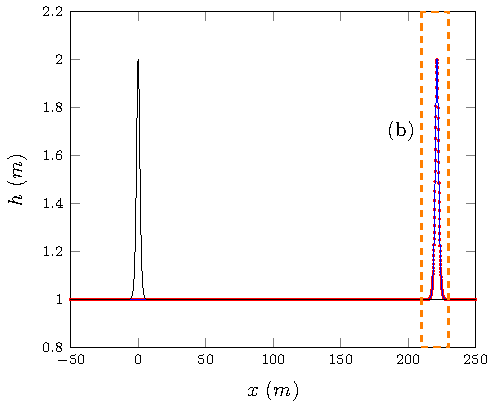
\includegraphics[width=7cm]{pics/results/soliton/ex/FDc.pdf}}
\subfigure[][]{\label{fig:FDsolhz} 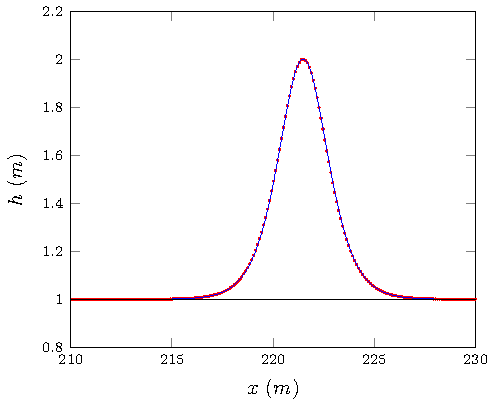
\includegraphics[width=7cm]{pics/results/soliton/ex/FDcz.pdf}}
\subfigure[][]{\label{fig:GRsolh}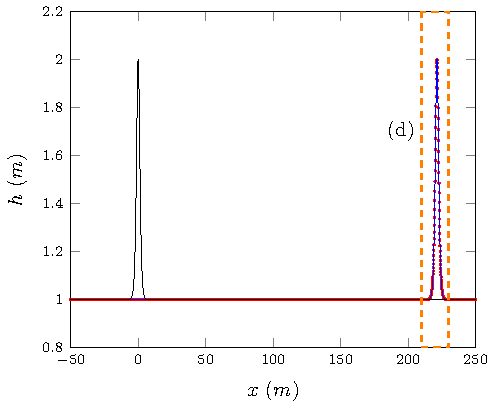
\includegraphics[width=7cm]{pics/results/soliton/ex/grim.pdf}}
\subfigure[][]{\label{fig:GRsolhz}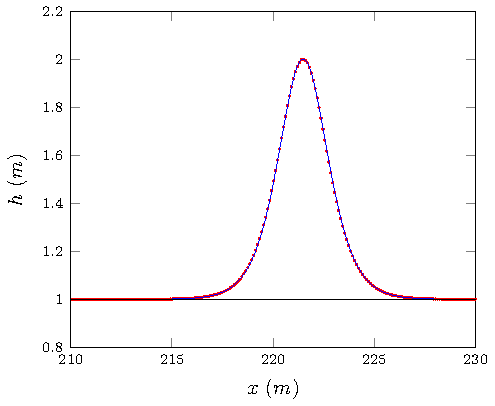
\includegraphics[width=7cm]{pics/results/soliton/ex/grimz.pdf}}
\caption{Water profile for the soliton problem \eqref{eq:sol} for $\mathcal{G}$ ((a),(b)) and $\mathcal{E}$ ((c),(d)) when $\Delta x = 10/2^{12}$ with the initial conditions ({\color{black} \solidrule}), analytic solution ({\color{blue} \solidrule}) and numerical result ({\color{red} $\bullet$}).}
\label{fig:FDMsolexp}
\end{figure}
\begin{figure}
\centering
\subfigure[][]{\label{fig:FDo2normL1}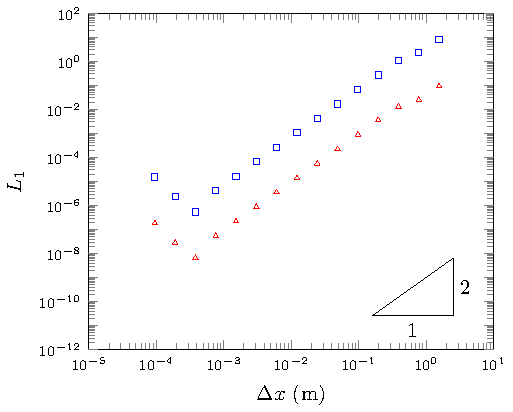
\includegraphics[width=7cm]{pics/results/soliton/L1/FDc.pdf}}
\subfigure[][]{\label{fig:FDo2Enorm}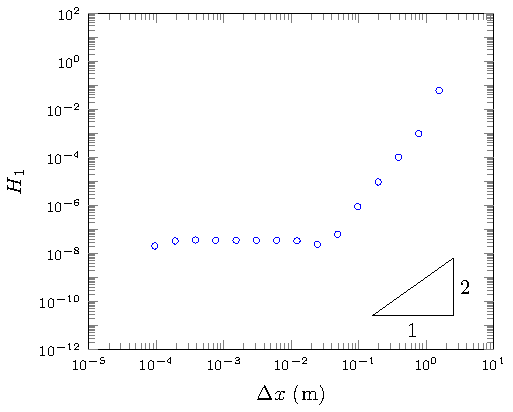
\includegraphics[width=7cm]{pics/results/soliton/H1/FDc.pdf}}
\subfigure[][]{\label{fig:grimo2normL1}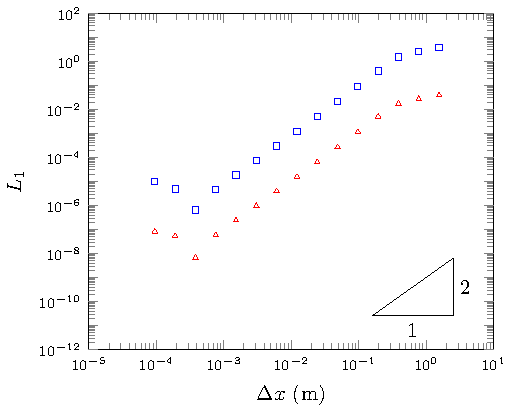
\includegraphics[width=7cm]{pics/results/soliton/L1/grim.pdf}}
\subfigure[][]{\label{fig:grimo2Enorm}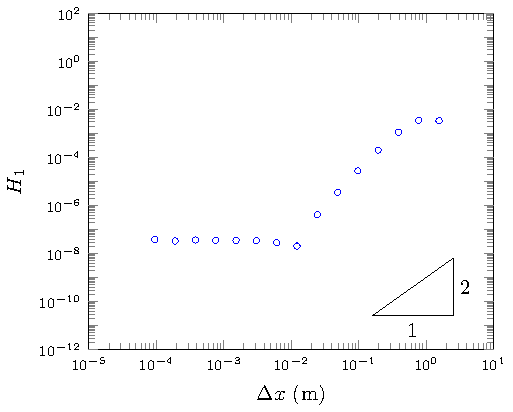
\includegraphics[width=7cm]{pics/results/soliton/H1/grim.pdf}}
\caption{On the left $L_1$ errors for $h$ ({\color{red} $\triangle$}) and $u$ ({\color{blue} $\square$}) and on the right $H_1$ ({\color{blue} $\circ$}) for the soliton problem with (a) and (b) for $\mathcal{G}$ and (c) and (d) for $\mathcal{E}$ .}
\label{fig:FDMsolnorm}
\end{figure}

\begin{figure}
\centering
\subfigure[][]{\label{fig:FDo2normC1}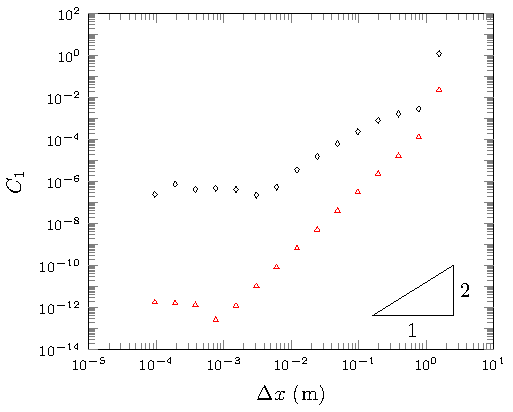
\includegraphics[width=7cm]{pics/results/soliton/C1/FDc.pdf}}
\subfigure[][]{\label{fig:grimo2normC1}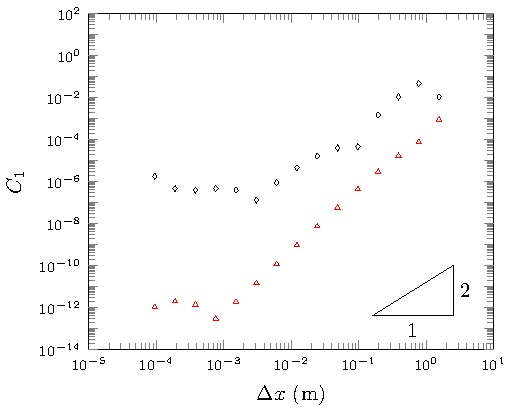
\includegraphics[width=7cm]{pics/results/soliton/C1/grim.pdf}}
\caption{$C_1$ for $h$ ({\color{red} $\triangle$}) and $uh$ ({\color{black} $\diamond$}) for numerical solutions $\mathcal{G}$ (a) and $\mathcal{E}$ (b) of the soliton problem.}
\label{fig:FDMsolnormC1}
\end{figure}
%
From Figure \ref{fig:FDMsolnorm} it can be seen that both FD methods are convergent under $L_1$ with second-order accuracy. In both $L_1$ plots the round-off effects for very small $\Delta x$ can be observed resulting in a loss of accuracy. For Figure \ref{fig:grimo2normL1} the effects of large $\Delta x$'s can be seen which is a suboptimal rate of convergence as the initial conditions cannot be accurately represented by the discretisation.

$H_1$ measures how well the method conserves the Hamiltonian, from Figures \ref{fig:FDo2Enorm} and \ref{fig:grimo2Enorm} we see that the FD methods conserve the Hamiltonian well and converge to the correct value of $0$ for $H_1$. Unfortunately, the point at which round off errors dominate is much earlier than for $L_1$ this is because the $H_1$ uses a very high order numerical integration calculation requiring more calculations than $L_1$ introducing more round off errors. $H_1$ also suffers from the same problems that $C
_1$ suffers as well leading to the stagnation of convergence seen in both. Although we do attain similar order of magnitudes for $L_1$ and $H_1$ before round off errors dominate. []

Lastly Figure \ref{fig:FDMsolnormC1} demonstrates conservation of both mass and momentum to at least second-order for both FD schemes. Both schemes conserve mass very well with round off error dominance occurring at the same place as for $L_1$. Momentum has the appropriate order of accuracy for larger $\Delta x$ but then stagnates as $\Delta x$ decreases. This is due to the use of a finite difference method which is not necessarily conservative on \eqref{eq:Serre_momentum} which is not in conservation law form leading to poor conservation of the momentum variable as compared to mass. Figure \ref{fig:FDMsolnormC1} however still demonstrates that these schemes are still relatively conservative and certainly there is not some drastic change in the momentum and mass in a system using these methods. 

These results demonstrate that these methods solve the Serre equations well and as such are appropriate to solve problems with smooth initial conditions. Because these methods do not require a reformulation, an elliptic solver or a bound on the wave speed these methods demonstrate that these added complexities are not the cause of the behaviours observed for the smooth dam break problem. Thus the observed behaviours are a property of the underlying equations and not the result of a particular numerical technique. 

%--------------------------------------------------------------------------------
\section{Smoothed Dam-Break}
\label{section:smootheddambreak}
%--------------------------------------------------------------------------------
The discontinuous dam-break problem can be approximated smoothly using the hyperbolic tangent function. Such an approximation will be called a smoothed dam-break problem and will be defined as such
\begin{linenomath*}
\begin{subequations}
\begin{gather}
h(x,0) = h_0 + \frac{h_1 - h_0}{2}\left(1 + \tanh\left(\alpha\left(x_0 - x\right)\right)\right),
\end{gather}
\begin{gather}
u(x,0) = 0.0m/s.
\end{gather}
\end{subequations}
\label{eq:sdbi}
\end{linenomath*}
Where $\alpha$ is given and controls the width of the transition between the two dam-break heights of $h_0$ and $h_1$. For large $\alpha$ the width is small and vice versa. We measure the transition width by taking the width of the dam break problem inside which $90 \%$ of the transition between the two states occurs which will be referred to as $\beta$. $\beta$ has the following formula independent of $h_0$, $h_1$ and $x_0$
\begin{linenomath*}
\begin{gather}
\beta = \frac{2 \tanh^{-1}\left(0.9\right)}{\alpha}.
\end{gather}
\label{eq:sdbtrans}
\end{linenomath*}

The dam break problem for the one dimensional Serre equations was analysed by \citeN{El-etal-2006} and an expression for the lead soliton amplitude of a bore was given as
\begin{linenomath*}
\begin{gather}
\frac{\Delta}{\left(a^+ + 1\right)^{1/4}} - \left(\frac{3}{4 -  \sqrt{a^+ + 1}}\right)^{21/10} \left(\frac{2}{1 + \sqrt{a^+ + 1}}\right)^{2/5} = 0
\label{eq:aplusdef}
\end{gather}
\end{linenomath*}
where $\Delta = h_1 / h_0$ and $a^+$ is the leading soliton amplitude. This measure will be used to verify that our results are sensible although as pointed out by \citeN{El-etal-2006} $a^+$ and the measured lead soliton amplitude of a numerical solution can differ. 

In the first series of experiments $h_0 = 1.0m$, $h_1 = 1.8m$ on $x \in [0m,1000m]$ for $t \in [0s,30s]$ with $x_0 = 500m$. This scenario replicates one presented by \citeN{El-etal-2006} and \citeN{Hank-etal-2010-2034} and as such serves as a comparison for the results of both with $\mathcal{E}$ and $\mathcal{G}$ and the $3$ different order FDVMs described in []. The simulations were run with various values of $\Delta x$ and $\beta$. To ensure stability, especially of both FD methods a very restrictive relation of $\Delta t = 0.01 \Delta x$ was chosen. For $\mathcal{V}_2$ $\theta = 1.2$. From this description we calculate the Hamiltonian at the initial time analytically

\begin{gather}
\label{eqn:HamilDBinit}
\mathcal{H} (0) = 10398.6 - 0.7848\times\left[\frac{2}{\alpha} \tanh\left(500 \alpha\right)\right],
\end{gather}
which will be used to verify the produced numerical results. Applying \eqref{eq:aplusdef} with analytic results of [] gives $\Delta = 1.36898 $ for the bore and thus $a^+ = 1.73640$ (5 decimal places).

\begin{figure}
\centering
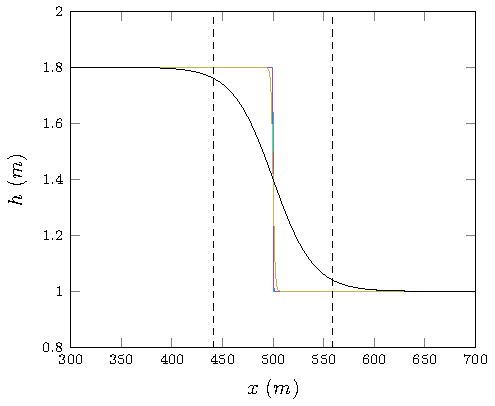
\includegraphics[width=7cm]{pics/results/SDB/init/h-figure0.pdf}
\caption{Initial conditions for the smooth dambreak problem with $\beta = 0.294$ ({\color{cyan!70!white} \solidrule}), $\beta = 1.17778$ ({\color{violet!70!white} \solidrule}), $\beta = 5.8888$ ({\color{yellow!70!black} \solidrule}) and  $\beta =117.778$ ({\color{black} \solidrule}) with reference $\beta$ interval({\color{black} \dashedrule}).}
\label{fig:dbsmoothinit}
\end{figure}

Figure \ref{fig:dbsmoothinit} shows the initial water profiles of smooth dam break problems with various $\beta$ values. It also indicates what the  $90 \%$ of the transition width for $\beta = 117.778$ is, with $90 \%$ capturing most of the transition. 

The following is an investigation into the results beginning with the behaviours of the solutions as $\Delta x  \rightarrow 0$. 

%--------------------------------------------------------------------------------
\subsection{Changing $\Delta x$}
%--------------------------------------------------------------------------------
Decreasing $\Delta x$ allows the numerical method to better approximate the analytic solution to the equations. So for our validated numerical methods it would be expected that smaller $\Delta x$'s provide a closer approximation to the analytic solution.

In this comparison we pick an $\beta$ and a method and investigate the result of decreasing $\Delta x$. Because the smoothness of the initial conditions depends on both $\Delta x$ and $\beta$ one must be careful that the initial conditions are sufficiently smooth as $\Delta x$ is decreased. This is of particular importance for the two finite difference methods as they do not correctly handle discontinuous initial conditions.

The first and most important observation is that there are four types of behaviour as $\Delta x \rightarrow 0$ depending on the $\beta$ and the numerical method. The four scenarios are identified by the behaviour of the solutions when $\Delta x$ is small and they correspond to different results in the literature. For brevity the only examples of these scenarios will the solutions of $\mathcal{V}_3$ although they all occurred for $\mathcal{V}_2$, $\mathcal{E}$ and $\mathcal{G}$ but not $\mathcal{V}_1$ which was too diffusive.

The first behaviour which will be referred to as the non-oscillatory scenario has such smooth initial conditions that no oscillations were introduced by $t= 30s$, although given sufficient time an undular bore would develop. An example of this behaviour was seen at $\beta = 117.778$ in Figure \ref{fig:o3a1dxlimflatexp}. Because this is a very smooth problem we observe rapid convergence with all the numerical results being graphically identical. This scenario resembles very diffusive solutions of the shallow water wave equations in that it contains only a rarefaction and a shock with no dispersive waves. 

This convergence is also present in Figure \ref{fig:o3a1dxlimmeasure} with both the $L_1$ and $H_1$ measures. Although now $L_1$ uses the solution of the smallest $\Delta x$ as an approximation to the analytic solution as none exists for this problem. In both measures the order of accuracy is the theoretical one, with round-off errors becoming dominant below $\Delta x = 0.1$. 

\begin{figure}
\centering
\subfigure[][]{\label{fig:o3a1dxlim}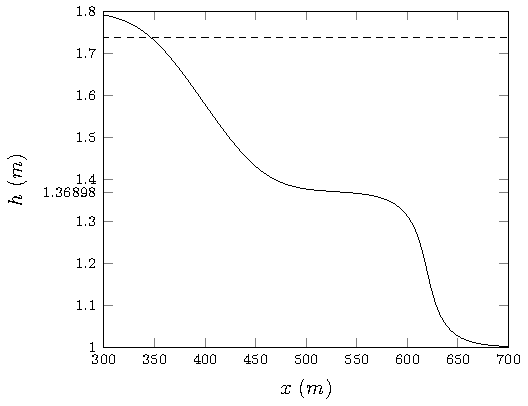
\includegraphics[width=7cm]{pics/results/SDB/numsols/alpha0.025/1-figure0.pdf}}
\caption{Numerical results of $\mathcal{V}_3$  at $t= 30s$ for the smooth dam break problem with $\beta =117.778$ for $\Delta x = 10/2^{10}$ ({\color{blue} \solidrule}), $\Delta x = 10/2^9$ ({\color{green!80!black} \solidrule}), $\Delta x = 10/2^8$ ({\color{red} \solidrule}), $\Delta x = 10/2^7$ ({\color{cyan!70!white} \solidrule}), $\Delta x = 10/2^6$ ({\color{violet!70!white} \solidrule}), $\Delta x = 10/2^5$ ({\color{yellow!70!black} \solidrule}), $\Delta x = 10/2^{4}$ ({\color{black} \solidrule}) with reference value $a^+$ ({\color{black} \dashedrule}).}
\label{fig:o3a1dxlimflatexp}
\end{figure}
%
\begin{figure}
\centering
\subfigure[][]{\label{fig:o3a1dxlimL1}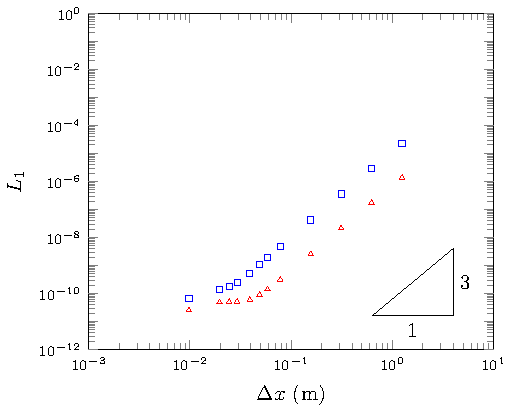
\includegraphics[width=7cm]{pics/results/SDB/Lcon/alpha0.025/1.pdf}}
\subfigure[][]{\label{fig:o3a1dxlimH}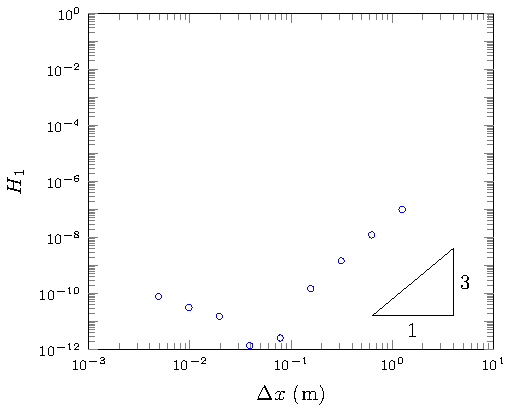
\includegraphics[width=7cm]{pics/results/SDB/Hcon/alpha0.025/1.pdf}}
\caption{$L_1$ for $h$ ({\color{red} $\triangle$}) and $u$ ({\color{blue} $\square$}) and $H_1$ ({\color{blue} $\circ$}) for $\mathcal{V}_3$'s solution for the smooth dambreak problem with $\beta =117.778$.}
\label{fig:o3a1dxlimmeasure}
\end{figure}

The second scenario will be referred to as the flat scenario due to the presence of a constant height state between the oscillations at the shock and rarefaction fan. An example of the numerical results for this scenario can be seen in Figure \ref{fig:o3a6dxlimflatexp} when $\beta = 5.8889$. This scenario corresponds to the results presented by \citeN{Hank-etal-2010-2034} and \citeN{Mitsotakis-etal-2014}. 

As $\Delta x$ decreases the solutions converge which is sensible since for the $\Delta x$ in Figure \ref{fig:o3a6dxlimflatexp} the initial conditions are smooth as can be seen in Figure \ref{fig:dbsmoothinit} and these methods have been verified for smooth problems. So that by $\Delta x = 10 / 2^8$ the solutions for higher $\Delta x$ are visually identical. 

The measures $L_1$ and $H_1$ also demonstrate good convergence with the expected order of convergence in the middle of the plot. Suboptimal convergence is expected for large $\Delta x$ as the problem is not properly discretised to resolve the oscillations and so both $H_1$ and $L_1$ suffer. For small $\Delta x$ $H_1$ becomes suboptimal suggesting significant round-off errors, however this effect is masked by $L_1$ because the smallest $\Delta x$ is has no comparsion and because it is based on comparison of two numerical simulations and not the analy

For the results in Figure \ref{fig:o3a6dxlimflatexp} the Hamiltonian for this problem is $10395.4608$(units).  The relative error for the conservation of the Hamiltonian by the third order method with $\Delta x = 10/2^{10}$ was $9.77469897234 \times 10^{-6}$. This low relative error suggests that our numerical method is solving the equations appropriately validating our results. We are however seeing the trend that will continue further on that our relative error is increasing as we better approximate the discontinuous initial conditions of the dam break problem.  


\begin{figure}
\centering
\subfigure[][]{\label{fig:o3a6dxlimz1}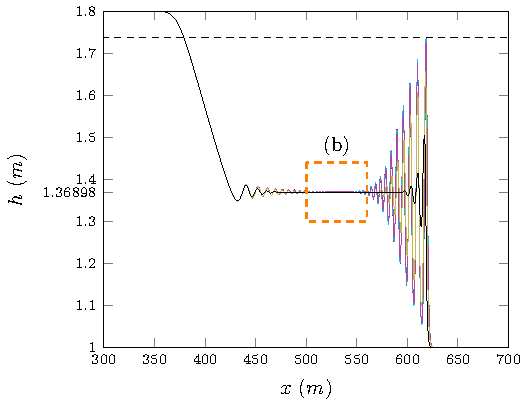
\includegraphics[width=7cm]{pics/results/SDB/numsols/alpha0.5/1-figure0.pdf}}
\subfigure[][]{\label{fig:o3a6dxlimz2}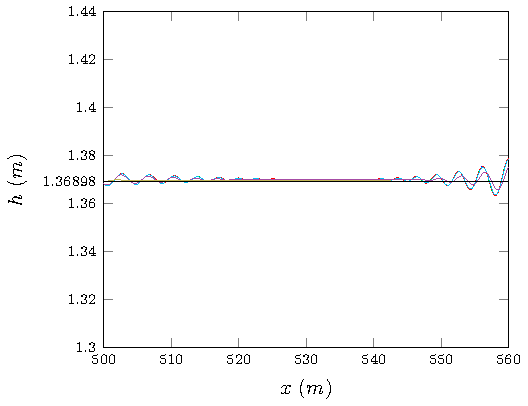
\includegraphics[width=7cm]{pics/results/SDB/numsols/alpha0.5/2-figure0.pdf}}
\caption{Numerical results of $\mathcal{V}_3$  at $t= 30s$ for the smooth dam break problem with $\beta = 5.8888$ for $\Delta x = 10/2^{10}$ ({\color{blue} \solidrule}), $\Delta x = 10/2^9$ ({\color{green!80!black} \solidrule}), $\Delta x = 10/2^8$ ({\color{red} \solidrule}), $\Delta x = 10/2^7$ ({\color{cyan!70!white} \solidrule}), $\Delta x = 10/2^6$ ({\color{violet!70!white} \solidrule}), $\Delta x = 10/2^5$ ({\color{yellow!70!black} \solidrule}), $\Delta x = 10/2^{4}$ ({\color{black} \solidrule}) with reference value $a^+$ ({\color{black} \dashedrule}).}
\label{fig:o3a6dxlimflatexp}
\end{figure}

\begin{figure}
\centering
\subfigure[][]{\label{fig:o3a2dxlimL1}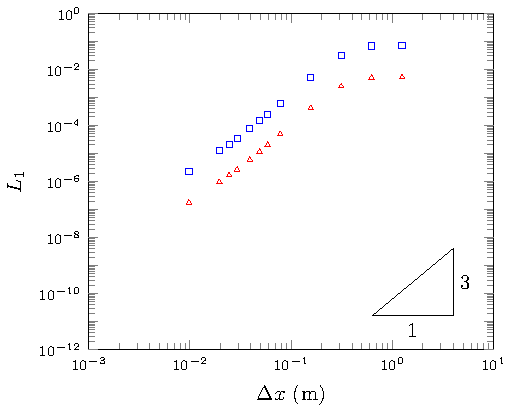
\includegraphics[width=7cm]{pics/results/SDB/Lcon/alpha0.5/1.pdf}}
\subfigure[][]{\label{fig:o3a2dxlimH}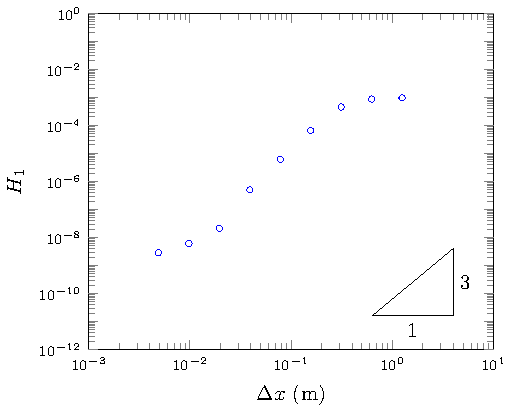
\includegraphics[width=7cm]{pics/results/SDB/Hcon/alpha0.5/1.pdf}}
\caption{$L_1$ for $h$ ({\color{red} $\triangle$}) and $u$ ({\color{blue} $\square$}) and $H_1$ ({\color{blue} $\circ$}) for $\mathcal{V}_3$'s solution for the smooth dambreak problem with $\beta = 5.8888$.}
\label{fig:o3a2dxlimmeasure}
\end{figure}

The third scenario will be referred to as the contact discontinuity scenario due to the use of that term to describe it by \citeN{El-etal-2006}. For the higher-order methods it occurs at $\alpha = 2.5$ and so far has not occurred for the first order method[]. The contact discontinuity scenarios main feature is that the oscillations from the rarefaction fan and the shock decay and appear to meet at a point as can be seen in Figure \ref{fig:o3a9dxlimcdexp}. For the experiments performed this doesn't appear to be an actual centre point but rather that the oscillations decay so quickly around the `contact discontinuity' that it appears to be the case. All the higher order methods so far have not shown a converged solution as $\Delta x$ decreases. However it does appear that convergence is likely with the solutions getting closer together. 

For the results in Figure \ref{fig:o3a9dxlimcdexp} the Hamiltonian of the initial conditions was calculated numerically to be $10397.97216$(units). The relative error for the conservation of the Hamiltonian by the third order method with $\Delta x = 10/2^{10}$ was $9.74612149745 \times 10^{-6}$. This shows that we are still accurately capturing the behaviour of the equations validating the of \citeN{El-etal-2006}. 


\begin{figure}
\centering
\subfigure[][]{\label{fig:o3a9dxlim}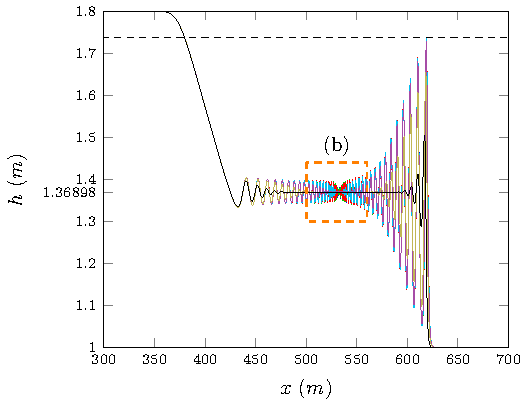
\includegraphics[width=7cm]{pics/results/SDB/numsols/alpha2.5/1-figure0.pdf}}
\subfigure[][]{\label{fig:o3a9dxlimz1}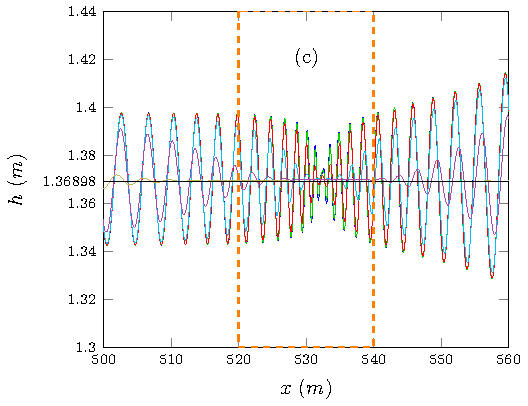
\includegraphics[width=7cm]{pics/results/SDB/numsols/alpha2.5/2-figure0.pdf}}
\subfigure[][]{\label{fig:o3a9dxlimz2}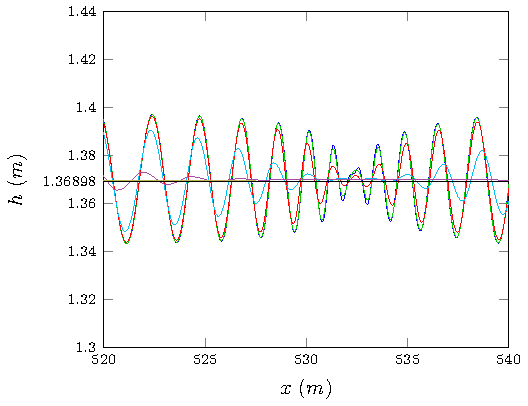
\includegraphics[width=7cm]{pics/results/SDB/numsols/alpha2.5/3-figure0.pdf}}
\caption{Numerical results of $\mathcal{V}_3$  at $t= 30s$ for the smooth dam break problem with $\beta = 1.17778$ for $\Delta x = 10/2^{10}$ ({\color{blue} \solidrule}), $\Delta x = 10/2^9$ ({\color{green!80!black} \solidrule}), $\Delta x = 10/2^8$ ({\color{red} \solidrule}), $\Delta x = 10/2^7$ ({\color{cyan!70!white} \solidrule}), $\Delta x = 10/2^6$ ({\color{violet!70!white} \solidrule}), $\Delta x = 10/2^5$ ({\color{yellow!70!black} \solidrule}), $\Delta x = 10/2^{4}$ ({\color{black} \solidrule}) with reference value $a^+$ ({\color{black} \dashedrule}).}
\label{fig:o3a9dxlimcdexp}
\end{figure}


\begin{figure}
\centering
\subfigure[][]{\label{fig:o3a3dxlimL1}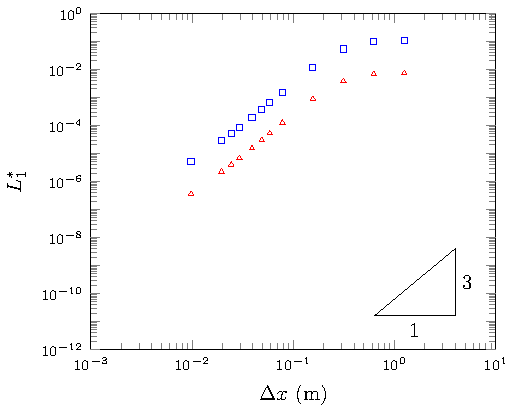
\includegraphics[width=7cm]{pics/results/SDB/Lcon/alpha2.5/1.pdf}}
\subfigure[][]{\label{fig:o3a3dxlimH}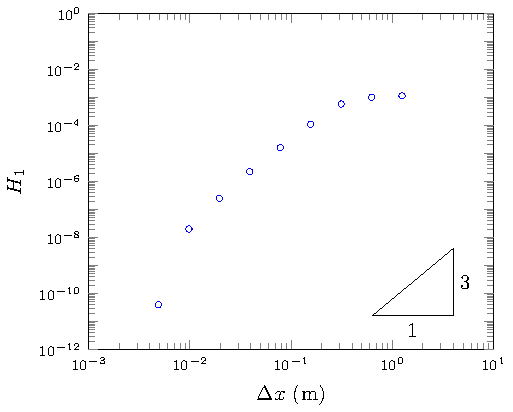
\includegraphics[width=7cm]{pics/results/SDB/Hcon/alpha2.5/1.pdf}}
\caption{$L^*_1$ for $h$ ({\color{red} $\triangle$}) and $u$ ({\color{blue} $\square$}) and $H_1$ ({\color{blue} $\circ$}) for $\mathcal{V}_3$'s solution for the smooth dambreak problem with $\beta = 1.17778$.}
\label{fig:o3a3dxlimmeasure}
\end{figure}

The fourth scenario will be referred to as the bump scenario due to the oscillations no longer decaying down towards a point but rather growing around where the contact discontinuity was in the previous scenario as can be seen in Figure \ref{fig:o3a20dxlimcdexp}. This behaviour has hitherto not been published and is certainly not an expected result. There are some important observations. Firstly changing $\alpha$ increases the height of the bump for the lowest resolution methods although after [] increasing $\alpha$ has no effect[huh?]. The behaviour of these solutions in Figure \ref{fig:o3a20dxlimcdexp} do not clearly show convergence.

For the results in Figure \ref{fig:o3a20dxlimcdexp} the Hamiltonian of the initial conditions was calculated numerically to be $10398.5984304$(units). The relative error for the conservation of the Hamiltonian by the third order method with $\Delta x = 10/2^{10}$ was $1.79088558176 \times 10^{-6}$. This shows that we are still accurately capturing the behaviour of the equations validating the of \citeN{El-etal-2006}.


\begin{figure}
\centering
\subfigure[][]{\label{fig:o3a20dxlim}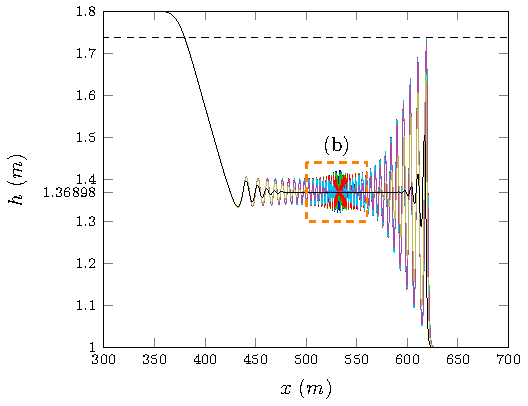
\includegraphics[width=7cm]{pics/results/SDB/numsols/alpha10/1-figure0.pdf}}
\subfigure[][]{\label{fig:o3a20dxlimz1}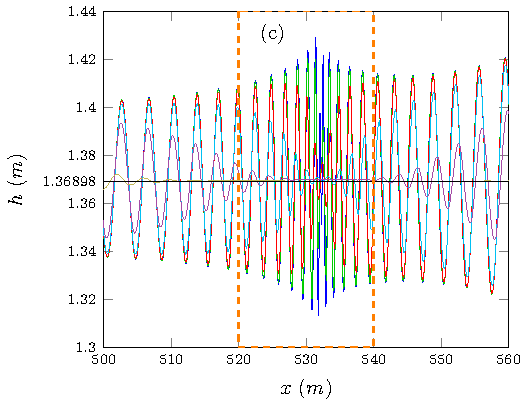
\includegraphics[width=7cm]{pics/results/SDB/numsols/alpha10/2-figure0.pdf}}
\subfigure[][]{\label{fig:o3a20dxlimz2}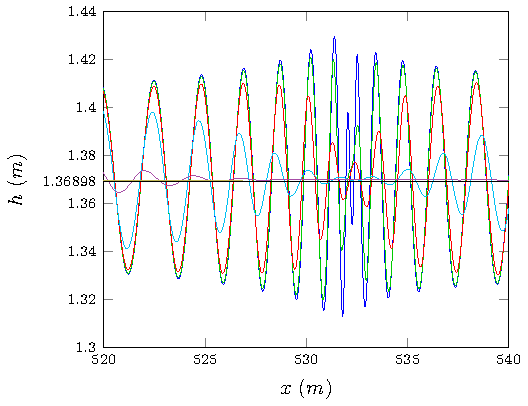
\includegraphics[width=7cm]{pics/results/SDB/numsols/alpha10/3-figure0.pdf}}
\caption{Numerical results of $\mathcal{V}_3$  at $t= 30s$ for the smooth dam break problem with $\beta = 0.294$ for $\Delta x = 10/2^{10}$ ({\color{blue} \solidrule}), $\Delta x = 10/2^9$ ({\color{green!80!black} \solidrule}), $\Delta x = 10/2^8$ ({\color{red} \solidrule}), $\Delta x = 10/2^7$ ({\color{cyan!70!white} \solidrule}), $\Delta x = 10/2^6$ ({\color{violet!70!white} \solidrule}), $\Delta x = 10/2^5$ ({\color{yellow!70!black} \solidrule}), $\Delta x = 10/2^{4}$ ({\color{black} \solidrule}) with reference value $a^+$ ({\color{black} \dashedrule}).}
\label{fig:o3a20dxlimcdexp}
\end{figure}


\begin{figure}
\centering
\subfigure[][]{\label{fig:o3a4dxlimL1}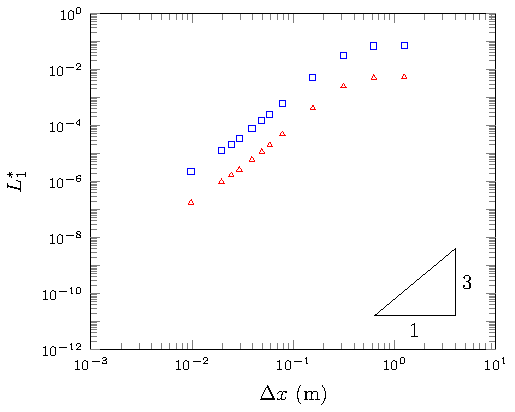
\includegraphics[width=7cm]{pics/results/SDB/Lcon/alpha10/1.pdf}}
\subfigure[][]{\label{fig:o3a4dxlimH}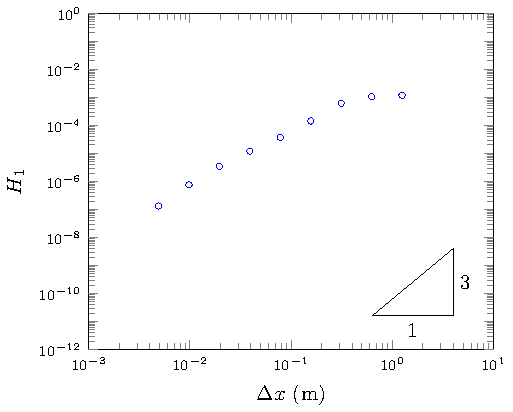
\includegraphics[width=7cm]{pics/results/SDB/Hcon/alpha10/1.pdf}}
\caption{$L^*_1$ for $h$ ({\color{red} $\triangle$}) and $u$ ({\color{blue} $\square$}) and $H_1$ ({\color{blue} $\circ$}) for $\mathcal{V}_3$'s solution for the smooth dambreak problem with $\beta = 0.294$.}
\label{fig:o3a4dxlimmeasure}
\end{figure}

\begin{figure}
\centering
\subfigure[][]{\label{fig:o3a4dxH1propFDVM}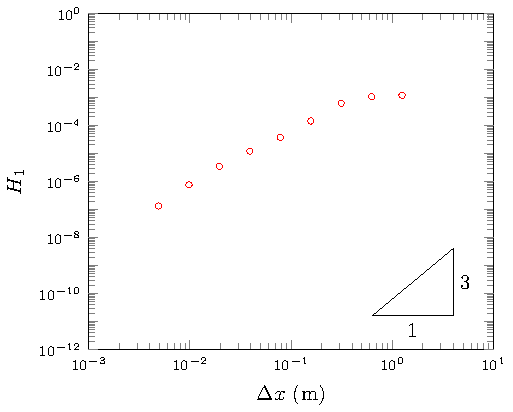
\includegraphics[width=7cm]{pics/results/SDB/Hcon/alpha10signs/o3.pdf}}
\subfigure[][]{\label{fig:o3a4dxH1propFD}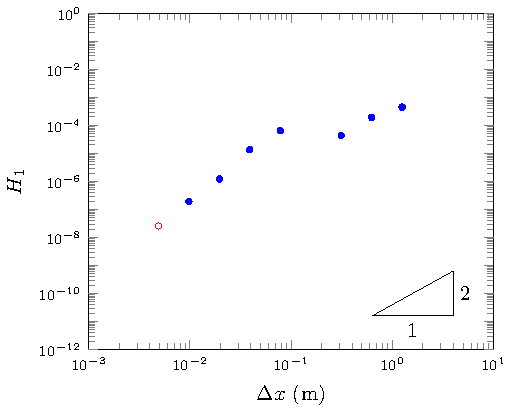
\includegraphics[width=7cm]{pics/results/SDB/Hcon/alpha10signs/FDc.pdf}}
\caption{$H_1$ for $\mathcal{V}_3$ (a) and $\mathcal{G}$'s (b) solution for the smooth dambreak problem at $t = 30s$ with $\beta = 0.294$ demonstrating when $\mathcal{H}(0s) \ge \mathcal{H}(30s)$ ({\color{red} $\circ$}) and $\mathcal{H}(0s) < \mathcal{H}(30s)$ ({\color{blue} $\bullet$}).}
\label{fig:o3a4dxHallsign}
\end{figure}

All of the scenarios described above and displayed using the higher-order FDVM also occur for the FDM, however because finite differences cannot properly handle discontinuities this is a little more subtle. Firstly, since for each $\alpha$ there is a $\Delta x$ such that for larger $\Delta x$ the smooth dam break problem is no longer smooth enough for a finite difference approximation to be appropriate. This becomes a problem for the contact discontinuity and bump scenarios since they require higher $\alpha$ and are thus are not very smooth to begin with. The result of this are non-physcial looking oscillations for large $\Delta x$ values that were not replicated by the FDVM and thus can be attributed to this flaw of FDM as in Figure \ref{fig:FDa20dxlimdexp}.

\begin{figure}
\centering
\subfigure[][]{\label{fig:FDa6h}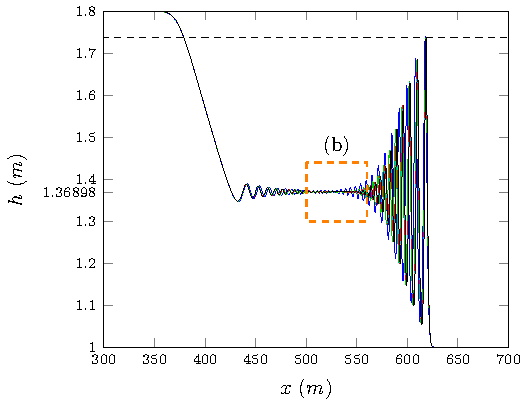
\includegraphics[width=7cm]{pics/results/SDB/numsols/FDcalpha0.5/1-figure0.pdf}}
\subfigure[][]{\label{fig:FDa6hz}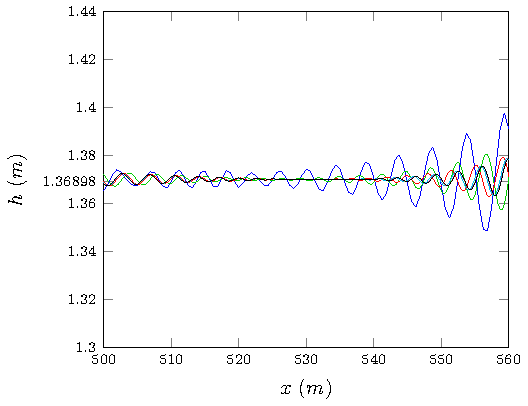
\includegraphics[width=7cm]{pics/results/SDB/numsols/FDcalpha0.5/2-figure0.pdf}}
\caption{Numerical results of $\mathcal{G}$  at $t= 30s$ for the smooth dam break problem with $\beta = 5.8888$ for $\Delta x = 10/2^{4}$ ({\color{blue} \solidrule}), $\Delta x = 10/2^5$ ({\color{green!80!black} \solidrule}), $\Delta x = 10/2^6$ ({\color{red} \solidrule}), $\Delta x = 10/2^7$ ({\color{cyan!70!white} \solidrule}), $\Delta x = 10/2^8$ ({\color{violet!70!white} \solidrule}), $\Delta x = 10/2^9$ ({\color{yellow!70!black} \solidrule}), $\Delta x = 10/2^{10}$ ({\color{black} \solidrule}) with reference value $a^+$ ({\color{black} \dashedrule})}
\label{fig:FDa6lim}
\end{figure}

\begin{figure}
\centering
\subfigure[][]{\label{fig:FDa12h}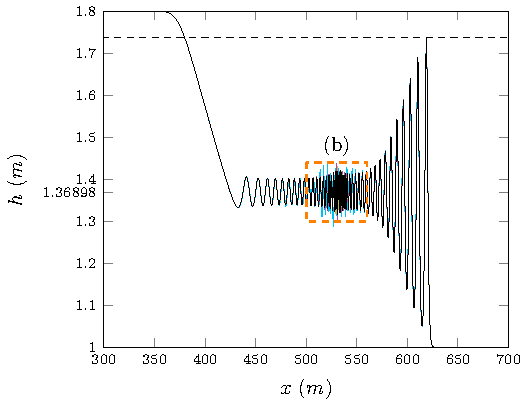
\includegraphics[width=7cm]{pics/results/SDB/numsols/FDcalpha10/1-figure0.pdf}}
\subfigure[][]{\label{fig:FDa12hz}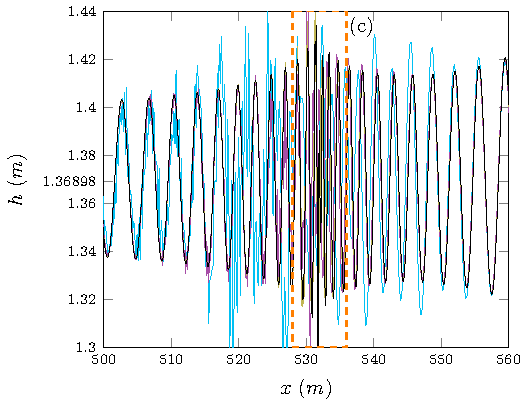
\includegraphics[width=7cm]{pics/results/SDB/numsols/FDcalpha10/2-figure0.pdf}}
\subfigure[][]{\label{fig:FDa12hzzz}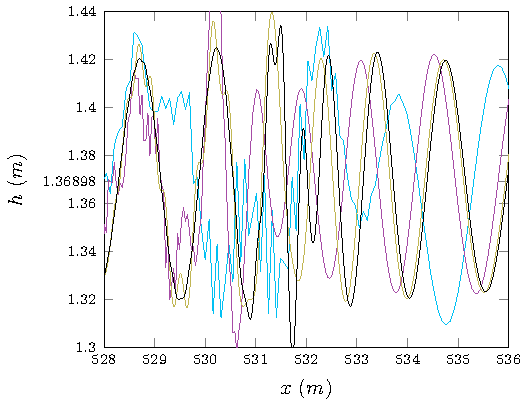
\includegraphics[width=7cm]{pics/results/SDB/numsols/FDcalpha10/4-figure0.pdf}}
\caption{Numerical results of $\mathcal{G}$  at $t= 30s$ for the smooth dam break problem with $\beta = 0.294$ for $\Delta x = 10/2^7$ ({\color{cyan!70!white} \solidrule}), $\Delta x = 10/2^8$ ({\color{violet!70!white} \solidrule}), $\Delta x = 10/2^9$ ({\color{yellow!70!black} \solidrule}), $\Delta x = 10/2^{10}$ ({\color{black} \solidrule}) with reference value $a^+$ ({\color{black} \dashedrule})}
\label{fig:FDa12lim}
\end{figure}
 

Overall there where two types of trending behaviours as $\Delta x$ was decreased one for the FDM and another for the FDVM. FDM decreased the number of oscillations in the solution as in Figure [], while FDVM increased the number of oscillations in the solution as can be seen in Figure []. This is explained by \citeN{Zoppou-Roberts-1996} as the FDM are second order finite difference approximations their errors are dissipative thus introducing oscillatory errors which are most prominent when $\Delta x$ and therefore the errors are large. While the behaviour of the FDVM is explained by a series of effects [] [TVD, treating things as cell averages, thus flattening things in cells,]. 

 
\begin{figure}
\centering
\subfigure[][]{\label{fig:FVlonga20h}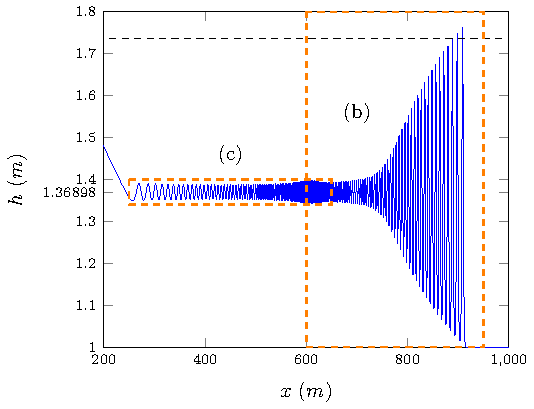
\includegraphics[width=7cm]{pics/results/SDB/numsols/longtime/hcrop-figure0.pdf}}
\subfigure[][]{\label{fig:FVlonga20hf}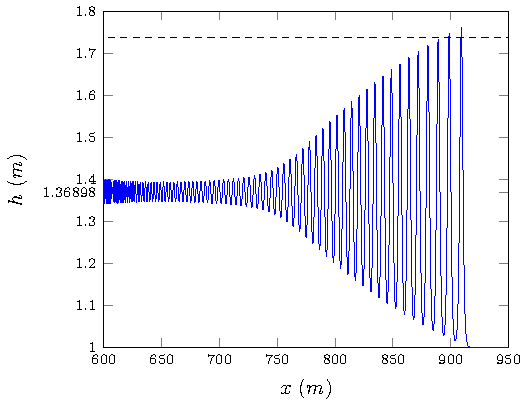
\includegraphics[width=7cm]{pics/results/SDB/numsols/longtime/hfront-figure0.pdf}}
\subfigure[][]{\label{fig:FVlonga20hb}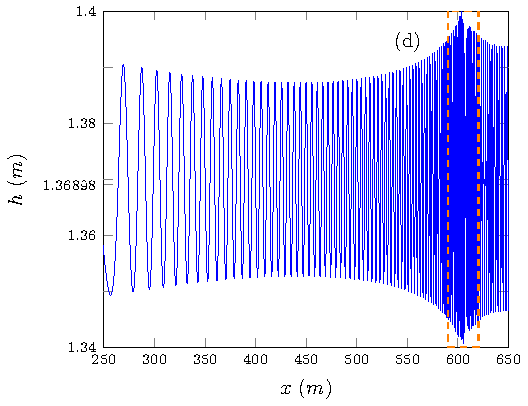
\includegraphics[width=7cm]{pics/results/SDB/numsols/longtime/hback-figure0.pdf}}
\subfigure[][]{\label{fig:FVlonga20hz}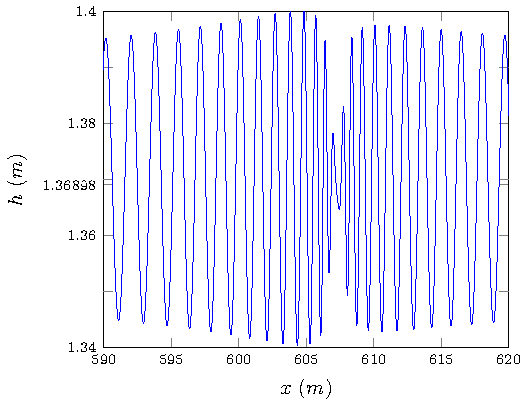
\includegraphics[width=7cm]{pics/results/SDB/numsols/longtime/hzz-figure0.pdf}}
\caption{Smooth dam break problem at $t=100s$ for $\mathcal{V}_3$ with $\beta = 0.294$ for $\Delta x = 10/2^{10}$ ({\color{blue} \solidrule}) with reference value $a^+$ ({\color{black} \dashedrule}).}
\label{fig:FVlonga20}
\end{figure}

\begin{figure}
\centering
\subfigure[][]{\label{fig:FVlonga20a}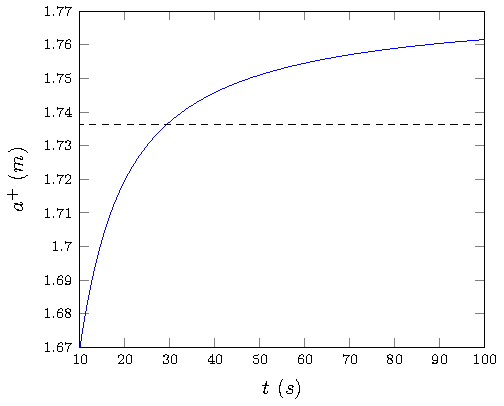
\includegraphics[width=7cm]{pics/results/SDB/numsols/longtime/a-figure0.pdf}}
\caption{Lead soliton height plotted over time for the smooth dam break problem at $t=100s$ for $\mathcal{V}_3$ with $\beta = 0.294$ for $\Delta x = 10/2^{10}$ ({\color{blue} \solidrule}) with reference value $a^+$ ({\color{black} \dashedrule}).}
\label{fig:FVlonga20aplus}
\end{figure}



%--------------------------------------------------------------------------------
\subsection{Changing $\alpha$}
%--------------------------------------------------------------------------------
Increasing $\alpha$ allows the initial conditions \eqref{eq:sdbi} to approach the dam break problem with $h_1$ to the left and $h_0$ to the right centred around $x_0$. So it would be expected that as $\alpha \rightarrow \infty$ that the solution of the smooth dam break problem would approach the corresponding dam break problem. This is the case for numerical methods because for a fixed $\Delta x$ $\alpha$ can be chosen large enough that \eqref{eq:sdbi} is precisely the dam break problem. This can be seen in Figure [] with $\Delta x =$ where the required $\alpha$ for this to occur is below $1000$ which was the maximum $\alpha$ value used in these experiments. However, only the FDVM were able to handle such large $\alpha$'s because the initial conditions are not smooth enough to allow for stability in the FDM as can be seen in Figure []. While the FDVM handled this quite well and for all $\Delta x$ tested as $\alpha$ increased the solutions converged, even though for higher $\Delta x$ [] $\alpha$ was not large enough to make \eqref{eq:sdbi} a jump discontinuity. 

This confirms the superiority of the FDVM to handle non smooth initial conditions and the inability of FDM to handle them. Even near discontinuous initial conditions caused problems for the FDM with the introduction of oscillations that were not replicated by the FDVM and appeared to be non-physical. An example of these transitional solutions between the properly smooth initial conditions and the unstable discontinuous ones can be seen in Figure []. [](only compare the models when FD started smooth enough)

For the range of $\alpha$'s which are smooth enough for the FDM to be appropriate then as $\alpha$ increases the number of oscillations increases as well for both the FDM and the FDVM. So that the smoothness of the initial conditions controls the oscillations but this depends on $\Delta x$ since for a fixed $\alpha$ the smoothness of the discretised initial conditions depends on $\Delta x$. [] (relative smoothness, more universal number)

It was observed that $\Delta x$ can be chosen large enough such that increasing $\alpha$ does not resolve some of the more complex structure observed for smaller $\Delta x$ values. This $\Delta x$ depends on the model most notably for the first-order finite difference-volume scheme this $\Delta x$ is very small. An example of this for the third-order FDVM scheme can be seen in Figure []. 



%--------------------------------------------------------------------------------
\subsection{Comparison of Models}
%--------------------------------------------------------------------------------
The first-order FDVM was too diffuse and

%--------------------------------------------------------------------------------
\subsection{Source}
%--------------------------------------------------------------------------------

%Scenario Comparison
\begin{figure}
\centering
\subfigure[][]{\label{fig:RFa12h}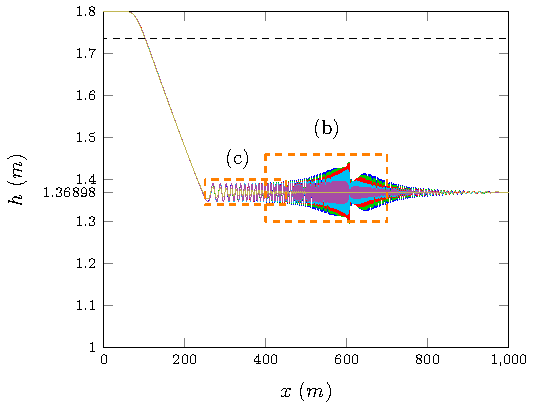
\includegraphics[width=7cm]{pics/results/SDB/DBSWcomp/all/RF1.pdf}}
\subfigure[][]{\label{fig:RFa12h2}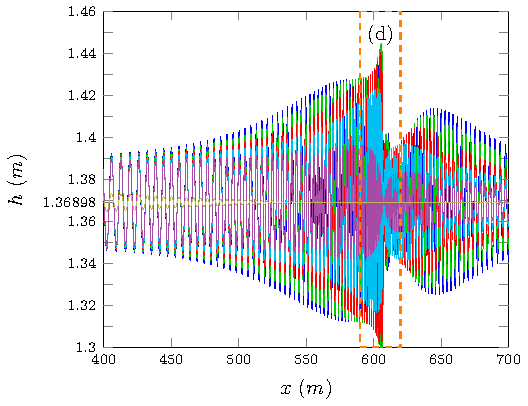
\includegraphics[width=7cm]{pics/results/SDB/DBSWcomp/all/RF3.pdf}}
\subfigure[][]{\label{fig:RFa12h3}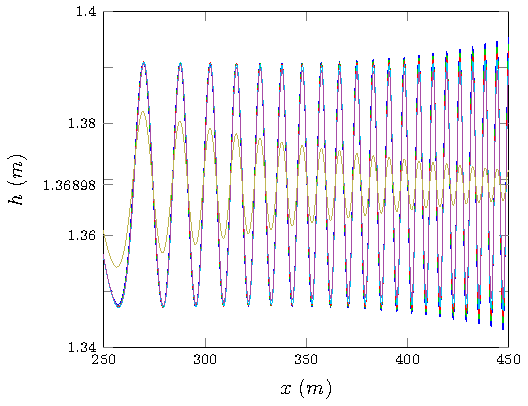
\includegraphics[width=7cm]{pics/results/SDB/DBSWcomp/all/RF4.pdf}}
\subfigure[][]{\label{fig:RFa12h4}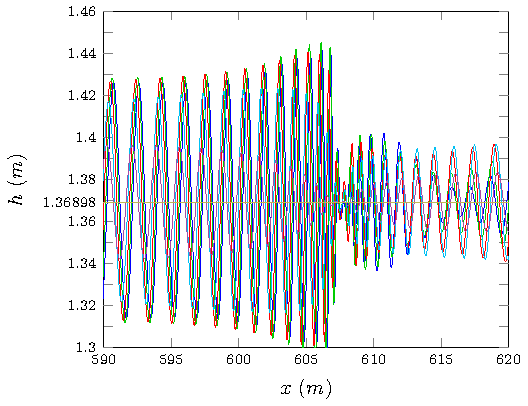
\includegraphics[width=7cm]{pics/results/SDB/DBSWcomp/all/RF6.pdf}}
\caption{Numerical results of $\mathcal{V}_3$  at $t= 100s$ for the smooth dam break rarefaction fan for $\Delta x = 10/2^{10}$ with $\beta = 0.2944$ ({\color{blue} \solidrule}), $\beta = 0.3464$ ({\color{green!80!black} \solidrule}), $\beta = 0.4530$ ({\color{red} \solidrule}), $\beta = 0.6543$ ({\color{cyan!70!white} \solidrule}) and $\beta = 1.1778$ ({\color{violet!70!white} \solidrule}) and $\beta = 5.8888$ ({\color{yellow!70!black} \solidrule}). }
\label{fig:RFa12hall}
\end{figure}

\begin{figure}
\centering
\subfigure[][]{\label{fig:SWa12h}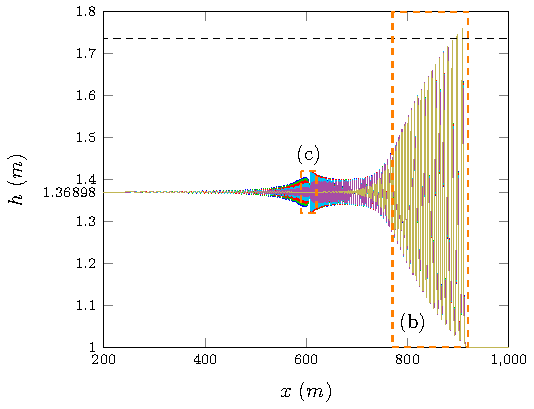
\includegraphics[width=7cm]{pics/results/SDB/DBSWcomp/all/SW1.pdf}}
\subfigure[][]{\label{fig:SWa12h3}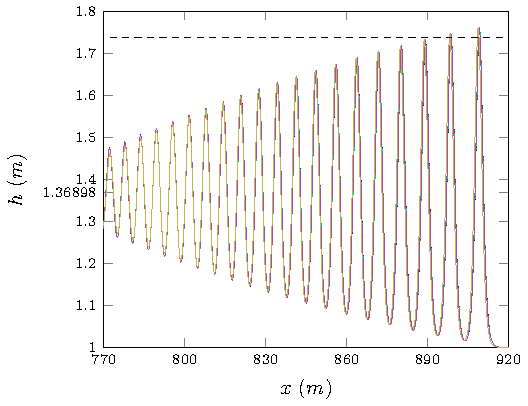
\includegraphics[width=7cm]{pics/results/SDB/DBSWcomp/all/SW2.pdf}}
\subfigure[][]{\label{fig:SWa12h4}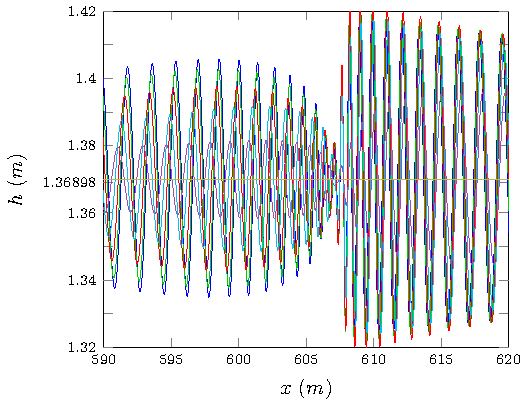
\includegraphics[width=7cm]{pics/results/SDB/DBSWcomp/all/SW5.pdf}}
\caption{Numerical results of $\mathcal{V}_3$  at $t= 100s$ for the smooth dam break shock wave for $\Delta x = 10/2^{10}$ with $\beta = 0.2944$ ({\color{blue} \solidrule}), $\beta = 0.3464$ ({\color{green!80!black} \solidrule}), $\beta = 0.4530$ ({\color{red} \solidrule}), $\beta = 0.6543$ ({\color{cyan!70!white} \solidrule}) and $\beta = 1.1778$ ({\color{violet!70!white} \solidrule}) and $\beta = 5.8888$ ({\color{yellow!70!black} \solidrule}). }
\label{fig:SWa12hall}
\end{figure}

\begin{figure}
\centering
\subfigure[][]{\label{fig:DBRFa12h}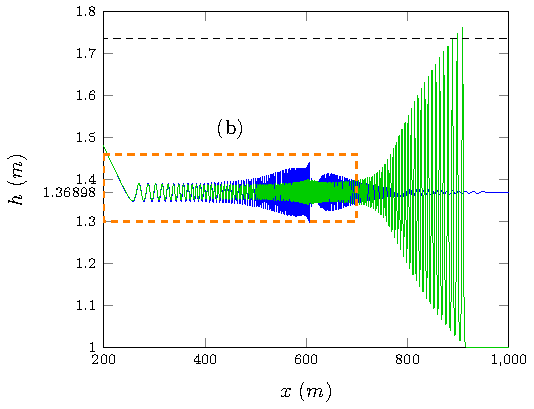
\includegraphics[width=7cm]{pics/results/SDB/DBSWcomp/long/RFlong1.pdf}}
\subfigure[][]{\label{fig:DBRFa12h2}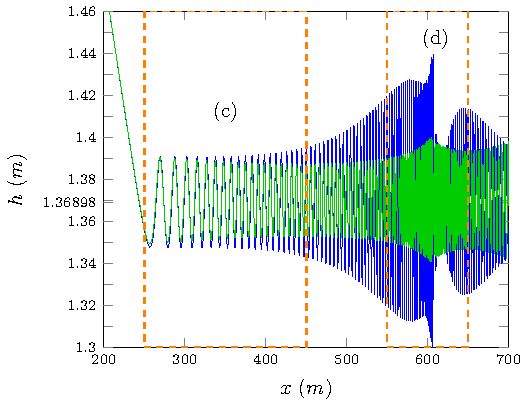
\includegraphics[width=7cm]{pics/results/SDB/DBSWcomp/long/RFlong2.pdf}}
\subfigure[][]{\label{fig:DBRFa12h3}\includegraphics[width=7cm]{pics/results/SDB/DBSWcomp/long/RFlong3.pdf}}
\subfigure[][]{\label{fig:DBRFa12h4}\includegraphics[width=7cm]{pics/results/SDB/DBSWcomp/long/RFlong4.pdf}}
\caption{Numerical results of $\mathcal{V}_3$  at $t= 100s$ for the smooth dam break $\beta = 0.2944$ ({\color{blue} \solidrule}) and the smooth dam break shock wave ({\color{green!80!black} \solidrule}), $\beta = 0.2944$ for $\Delta x = 10/2^{10}$. }
\label{fig:DBRFa12hall}
\end{figure}

\begin{figure}
\centering
\subfigure[][]{\label{fig:DBSWa12h}\includegraphics[width=7cm]{pics/results/SDB/DBSWcomp/long/SWlong1.pdf}}
\subfigure[][]{\label{fig:DBSWa12h3}\includegraphics[width=7cm]{pics/results/SDB/DBSWcomp/long/SWlong3.pdf}}
\subfigure[][]{\label{fig:DBSWa12h4}\includegraphics[width=7cm]{pics/results/SDB/DBSWcomp/long/SWlong4.pdf}}
\caption{Numerical results of $\mathcal{V}_3$  at $t= 100s$ for the smooth dam break $\beta = 0.2944$ ({\color{blue} \solidrule}) and the smooth dam break shock wave $\beta = 0.2944$({\color{green!80!black} \solidrule}) for $\Delta x = 10/2^{10}$. }
\label{fig:DBSWa12hall}
\end{figure}


%Energy
\begin{figure}
\centering
\subfigure[][]{\label{fig:HFTa12long}\includegraphics[width=7cm]{pics/results/SDB/H/long/HFT-figure0.pdf}}
\subfigure[][]{\label{fig:HFTa12zflong}\includegraphics[width=7cm]{pics/results/SDB/H/long/HFTzf-figure0.pdf}}
\subfigure[][]{\label{fig:HFTa12zzlong}\includegraphics[width=7cm]{pics/results/SDB/H/long/HFTzz-figure0.pdf}}
\caption{$\mathcal{H}_1$ for $\mathcal{V}_3$ solution of the smooth dam break with $\beta = 0.2944$ and $\Delta x = 10/2^{10}$ at $t=0s$ ({\color{blue} \solidrule}) and $t=100s$ ({\color{green!80!black} \solidrule}). }
\label{fig:HFTa12longall}
\end{figure}

\begin{figure}
\centering
\subfigure[][]{\label{fig:HSTa12long}\includegraphics[width=7cm]{pics/results/SDB/H/long/HST-figure0.pdf}}
\subfigure[][]{\label{fig:HSTa12zzzlong}\includegraphics[width=7cm]{pics/results/SDB/H/long/HSTzzz-figure0.pdf}}
\caption{$\mathcal{H}_2$ for $\mathcal{V}_3$ solution of the smooth dam break with $\beta = 0.2944$ and $\Delta x = 10/2^{10}$ at $t=0s$ ({\color{blue} \solidrule}) and $t=100s$ ({\color{green!80!black} \solidrule}). }
\label{fig:HSTa12longall}
\end{figure}

\begin{figure}
\centering
\subfigure[][]{\label{fig:HTTa12long}\includegraphics[width=7cm]{pics/results/SDB/H/long/HTT-figure0.pdf}}
\subfigure[][]{\label{fig:HTTa12zzlong}\includegraphics[width=7cm]{pics/results/SDB/H/long/HTTzf-figure0.pdf}}
\subfigure[][]{\label{fig:HTTa12zzzlong}\includegraphics[width=7cm]{pics/results/SDB/H/long/HTTzz-figure0.pdf}}
\caption{$\mathcal{H}_3$ for $\mathcal{V}_3$ solution of the smooth dam break with $\beta = 0.2944$ and $\Delta x = 10/2^{10}$ at $t=0s$ ({\color{blue} \solidrule}) and $t=100s$ ({\color{green!80!black} \solidrule}). }
\label{fig:HTTa12longall}
\end{figure}



\begin{figure}
\centering
\subfigure[][]{\label{fig:PHTa12}\includegraphics[width=7cm]{pics/results/SDB/H/Time/HFT-figure0.pdf}}
\subfigure[][]{\label{fig:PHTa12z}\includegraphics[width=7cm]{pics/results/SDB/H/Time/TT-figure0.pdf}}
\caption{Proportion of $\mathcal{H}$ made up by $\mathcal{H}_1$ ({\color{blue} \solidrule}) , $\mathcal{H}_2$ ({\color{green!80!black} \solidrule}) and $\mathcal{H}_3$ ({\color{red} \solidrule})  for $\mathcal{V}_3$ solution of the smooth dam break with $\beta = 0.2944$ and $\Delta x = 10/2^{10}$ over time.}
\label{fig:PHTa12all}
\end{figure}

%uh comparison
\begin{figure}
\centering
\subfigure[][]{\label{fig:UHcomp1}\includegraphics[width=7cm]{pics/results/SDB/UHcomp/0-figure0.pdf}}
\subfigure[][]{\label{fig:UHcomp2}\includegraphics[width=7cm]{pics/results/SDB/UHcomp/2-figure0.pdf}}
\subfigure[][]{\label{fig:UHcomp3}\includegraphics[width=7cm]{pics/results/SDB/UHcomp/3-figure0.pdf}}
\subfigure[][]{\label{fig:UHcomp4}\includegraphics[width=7cm]{pics/results/SDB/UHcomp/5-figure0.pdf}}
\caption{$h$ ({\color{blue} \solidrule}) and adjusted $u$ ({\color{green!80!black} \solidrule})  for $\mathcal{V}_3$ solution of the smooth dam break with $\beta = 0.2944$ and $\Delta x = 10/2^{10}$ at $t=100s$. }
\label{fig:UHcompall}
\end{figure}

%cd speed
\begin{figure}
\centering
\subfigure[][]{\label{fig:CDspeed1}\includegraphics[width=7cm]{pics/results/SDB/CDspeed/speed.pdf}}
\caption{$v_{DB}$ ({\color{blue} \solidrule}) and $v_{CD}$ ({\color{red} $\circ$})  for $\mathcal{V}_3$ solution of the various smooth dam break problems with $\beta = 0.2944$ and $\Delta x = 10/2^{10}$ at $t=100s$. }
\label{fig:CDspeed}
\end{figure}




%\subsection{Dam-Break} %old
%--------------------------------------------------------------------------------
%The dam-break problem can be defined as such
%\begin{linenomath*}
%\begin{gather*}
%h(x,0) = \left\lbrace \begin{array}{c c}
%1.8 & x < 500\\
%1.0 & x \ge 500\\
%\end{array} \right. ,
%\end{gather*}
%\begin{gather*}
%u(x,0) = 0.0m/s.
%\end{gather*}
%\end{linenomath*}
%With $x \in \left[0\text{m},1000\text{m}\right]$ for $t \in \left[0\text{s},30\text{s}\right]$. Where $\lambda = 0.01 \text{m/s}$ and $\theta = 1.2$. This corresponds to sub-critical flow and was a situation demonstrated in \citeN{El-etal-2006} and \citeN{Hank-etal-2010-2034}. An example was plotted for %$\Delta x = 100 /2^{10}\text{m}$ for all the methods and for $\Delta x = 100 %/2^{15}\text{m}$ for the first-order method in Figure \ref{fig:DB}. To determine if %the oscillations that occur in the solution indeed converge to some limit as $\Delta x %\rightarrow 0$ multiple $\Delta x$ values were run and then the amount of variation in %the solution measured. This measured how oscillatory the solution was and was used to %determine the growth of the oscillations. A common way to measure this is the total %variation $TV$ \cite{LeVeque-2002} which for $\boldsymbol{q}$ is given by
%\begin{linenomath*}
%\begin{gather*}
%TV(\boldsymbol{q}) = \sum_{\forall i >1} |q_{i} - q_{i-1}|.
%\end{gather*}
%\end{linenomath*}
%If the solution does indeed converge then the TV must at some point plateau, bounding the oscillations. This was indeed the findings of the experiments as can be seen by Figure \ref{fig:DBL1}. The TV increases as $\Delta x$ decreased because the models resolved more dispersive waves. As $\Delta x$ decreased further the TV plateaued and so the size and number of oscillations was bounded. Therefore, the scheme has not become unstable which supports the argument that the numerical schemes do not introduce non-physical oscillations in the solution. The second-order scheme converges rapidly to the solution of the third-order scheme.

%\begin{figure}
%\begin{center}
%\includegraphics[width=8.0cm]{./results/dambreak/L1con/both-figure0.pdf}
%\end{center}
%\caption{The change in total variation (TV) over $\Delta x$ for; ($\circ$) first- , %($\square$) second-, and ($*$) third-order schemes.}
%\label{fig:DBL1}
%\end{figure}
%\begin{figure}
%\centering
%\subfigure[][]{\label{fig:DBo1}\includegraphics[width=7cm]{./results/dambreak/ex/o1-figure0.pdf}}
%\subfigure[][]{\label{fig:DBo2}\includegraphics[width=7cm]{./results/dambreak/ex/o2-figure0.pdf}}
%\subfigure[][]{\label{fig:DBo3}\includegraphics[width=7cm]{./results/dambreak/ex/o3-figure0.pdf}}
%\subfigure[][]{\label{fig:DB1o1}\includegraphics[width=7cm]{./results/dambreak/ex/o1-figure1.pdf}}
%\caption{Solution of the dam-break problem using the (a) first-, (b) second- and (c) third-order method with $\Delta x = 100 /2^{10} \text{m}$. As well as a (d) first-order method with $\Delta x = 100 /2^{15} \text{m}$. }
%\label{fig:DB}
%\end{figure}

%These solutions compare very well to the findings in \citeN{El-etal-2006} with both the second- and third-order schemes resolving the oscillations around the "contact discontinuity"\cite{El-etal-2006} between the rarefaction fan and the shock. In \citeN{Hank-etal-2010-2034} it was reported that for their first-order scheme such oscillatory behaviour was not seen. However, for the first-order scheme proposed in this paper when $\Delta x = 100 /2^{15}$ it was resolved as in Figure \ref{fig:DB1o1}. This validates the findings in \citeN{El-etal-2006}.

%There is also a good agreement between the second- and third-order simulations of the dam-break problem as can be seen in Figures \ref{fig:DBo2} and \ref{fig:DBo3}. Although more oscillations are resolved by the third-order scheme over the second-order scheme, there is no significant change in the resolved behaviour of this problem between the two schemes. As noted in the introduction second-order errors are dissipative; since the diffusive third-order scheme resolved the same oscillations it was demonstrated that none of the dissipative errors significantly polluted the wave train and so the second-order scheme is capable of resolving the problem well.
%--------------------------------------------------------------------------------
\section{Conclusions}
\label{section:Conclusions}
%--------------------------------------------------------------------------------

%--------------------------------------------------------------------------------
\section{Acknowledgements}
%--------------------------------------------------------------------------------

%--------------------------------------------------------------------------------
\bibliography{Serre_ASCE}
%--------------------------------------------------------------------------------

\end{document}
